\documentclass[11pt,table]{beamer}
\mode<presentation>
\usepackage{etex}
\usepackage{graphicx}
\usepackage{epstopdf}
\usepackage[english]{babel}
\usepackage{tabularx}
\usepackage{booktabs}
\usepackage{mathrsfs}
\usepackage{multicol}
\usepackage{bm}
\usepackage{subcaption}
\usepackage{wrapfig}
\usepackage{dcolumn}
\usepackage{threeparttable}
\usepackage{booktabs}
\usepackage{bbm}
\usepackage{amsmath,dsfont,listings}
\usepackage{amssymb}
\usepackage{rotating}
\usepackage{multirow}
\usepackage{tcolorbox}
\usepackage[authoryear]{natbib}
\usepackage{circledsteps}
\usepackage{qtree}

\usepackage{tikz}
\usetikzlibrary{arrows,decorations.pathmorphing,backgrounds,fit,positioning,shapes.symbols,chains}
\usetikzlibrary{arrows.meta, calc}

\setbeamertemplate{section in toc}[sections numbered]
\setbeamertemplate{caption}[numbered]

\bibliographystyle{Econometrica}

\setbeamersize{text margin right=3.5mm, text margin left=7.5mm}  % text margin
\setbeamersize{sidebar width left=0cm, sidebar width right=0mm}
\setbeamertemplate{sidebar right}{}
\setbeamertemplate{sidebar left}{}

\definecolor{text-grey}{rgb}{0.45, 0.45, 0.45} % grey text on white background
\definecolor{bg-grey}{rgb}{0.66, 0.65, 0.60} % grey background (for white text)
\definecolor{fu-blue}{RGB}{0, 51, 102} % blue text
\definecolor{fu-green}{RGB}{153, 204, 0} % green text
\definecolor{fu-red}{RGB}{204, 0, 0} % red text (used by \alert)
\definecolor{bluegray}{HTML}{B9CDE5}
\definecolor{BrewerBlue}{HTML}{377EB8} % Define Brewer Blue
\definecolor{BrewerRed}{HTML}{E41A1C}  % Define Brewer Red

\setbeamertemplate{frametitle}{%
    \vskip-30pt \color{text-grey}\large%
    \begin{minipage}[b][23pt]{\textwidth}%
    \flushleft\insertframetitle%
    \end{minipage}%
}

\setbeamertemplate{navigation symbols}{} 

%%% begin title page
\setbeamertemplate{title page}{
\vskip2pt\hfill
\vskip19pt\hskip3pt

% set the title and the author
\vskip4pt
\parbox[top][1.35cm][c]{11cm}{\LARGE\color{text-grey} \textcolor{red1}{RL}earning:\\[1ex] \inserttitle \\[1ex] \small \quad \\[3ex]}
\vskip17pt
\parbox[top][1.35cm][c]{11cm}{\small  \insertsubtitle \\[2ex] \insertauthor \\[1ex]}
}
%%% end title page

%%% colors
\usecolortheme{lily}
\setbeamercolor*{normal text}{fg=black,bg=white}
\setbeamercolor*{alerted text}{fg=fu-red}
\setbeamercolor*{example text}{fg=fu-green}
\setbeamercolor*{structure}{fg=fu-blue}

\setbeamercolor*{block title}{fg=white,bg=black!50}
\setbeamercolor*{block title alerted}{fg=white,bg=black!50}
\setbeamercolor*{block title example}{fg=white,bg=black!50}

\setbeamercolor*{block body}{bg=black!10}
\setbeamercolor*{block body alerted}{bg=black!10}
\setbeamercolor*{block body example}{bg=black!10}

\setbeamercolor{bibliography entry author}{fg=fu-blue}
\setbeamercolor{bibliography entry journal}{fg=text-grey}
\setbeamercolor{item}{fg=fu-blue}
\setbeamercolor{navigation symbols}{fg=text-grey,bg=bg-grey}
%%% end colors

%%% headline
\setbeamertemplate{headline}{
\vskip30pt
}
%%% end headline

%%% footline
\newcommand{\footlinetext}{
%\insertshortinstitute, \insertshorttitle, \insertshortdate
}
\setbeamertemplate{footline}{
\vskip2pt
\hfill \raisebox{-1pt}{\usebeamertemplate***{navigation symbols}}
\hfill \insertframenumber\hspace{10pt}
\vskip4pt
}
%%% end footline

%%% settings for listings package
\lstset{extendedchars=true, showstringspaces=false, basicstyle=\footnotesize\sffamily, tabsize=2, breaklines=true, breakindent=10pt, frame=l, columns=fullflexible}
\lstset{language=Java} % this sets the syntax highlighting
\lstset{mathescape=true} % this switches on $...$ substitution in code
% enables UTF-8 in source code:
\lstset{literate={ä}{{\"a}}1 {ö}{{\"o}}1 {ü}{{\"u}}1 {Ä}{{\"A}}1 {Ö}{{\"O}}1 {Ü}{{\"U}}1 {ß}{\ss}1}
%%% end listings

\usepackage{concmath}
\usepackage{xcolor}
\definecolor{red1}{RGB}{206, 17, 38}
\definecolor{blue1}{RGB}{16, 118, 208}
\definecolor{gray1}{RGB}{117, 115, 115}
\usepackage{hyperref}


\newtheorem{proposition}{Proposition}
\newtheorem{assumption}{Definition}

\title[]{Short guides to reinforcement learning}
\subtitle[]{Introduction}
\author[D. Rostam-Afschar]{\textcolor{gray1}{Davud Rostam-Afschar (Uni Mannheim)}}
\date[]{\today}
\subject{Econometrics}
\renewcommand{\footlinetext}{\insertshortinstitute, \insertshorttitle, \insertshortdate}
\hypersetup{
    bookmarks=false,
    unicode=false,
    pdftoolbar=false,
    pdffitwindow=true,
    pdftitle={Reinforcement Learning for Business, Economics, and Social Sciences: \insertsubtitle},
    pdfauthor={Davud Rostam-Afschar},
    pdfsubject={Reinforcement Learning},
    pdfkeywords={Intro},
    pdfnewwindow=true,
}
\def\sym#1{\ifmmode^{#1}\else\(^{#1}\)\fi}

\begin{document}

\begin{frame}[plain]
  \titlepage
\end{frame}

% --------------------------------------------------- Slide --
%\begin{frame}
	%\frametitle{Content}
	%\tableofcontents[]
%\end{frame}

\section{Introduction to Reinforcement Learning}
{
\setbeamercolor{background canvas}{bg=BrewerBlue}
\begin{frame}
\centering
\Huge
\textcolor{white}{What is Reinforcement Learning?}
\thispagestyle{empty}
\end{frame}
}


\begin{frame}{Machine Learning}

\begin{columns}[T]
\begin{column}{0.6\textwidth}
\begin{itemize}
    \item Traditional computer science
\begin{itemize}
    \item Program computer for every task \pause
\end{itemize}
\end{itemize}
\end{column}
\begin{column}{0.4\textwidth}
\centering
\includegraphics[width=0.8\textwidth]{figures/programmer}
\end{column}
\end{columns}\pause
    \begin{itemize}
        \item New paradigm
\begin{itemize}
    \item Provide examples to machine
\item Machine learns to accomplish a task based on the  examples
 
\end{itemize}

    \end{itemize}

\begin{columns}[T]
\begin{column}{0.5\textwidth}
\pause\centering
\includegraphics[width=0.9\textwidth]{figures/sample translations} % Sample translations made by the neural machine translation model with the soft-attention mechanism. Edge thicknesses represent the attention weights found by the attention model. Kyunghyun Cho, 2015
\end{column}
\begin{column}{0.5\textwidth}
\centering \pause
\includegraphics[width=0.8\textwidth]{figures/yolov7e6.png}
\end{column}
\end{columns}


\end{frame}

\begin{frame}{Machine Learning: Different Approaches}

\begin{itemize}
    \item \textbf{Supervised Learning}
    \begin{itemize}
        \item Most common type of machine learning
        \item Learns from labeled examples\\ (input + correct output)
        \pause
        \item \textbf{Challenge:} Needs lots of labeled data 
    \end{itemize}
    \pause
\end{itemize}

\only<1-2>{
\vspace*{13.6em}
\quad
}

\only<3>{
\begin{center}
\includegraphics[width=0.3\linewidth]{figures/selectallsquareswithvehicles.jpg}
\end{center}
}


\only<4->{\vspace{2em}
\begin{itemize}
    \item \textbf{Other Approaches}
    \begin{itemize}
        \item \textbf{Unsupervised Learning:}\\ Finds patterns without labeled data
        \item \textbf{Semi-supervised Learning:}\\ Mixes labeled and unlabeled data
        \item \textcolor{red1}{\textbf{Reinforcement Learning:}}\\ Learns by trial and error
    \end{itemize}
\end{itemize}\vspace{4.3em}
}

\end{frame}

\begin{frame}{Animal Psychology}

\begin{columns}[T]
\begin{column}{0.6\textwidth}
\begin{itemize}

    \item Positive reinforcements:
    \begin{itemize}
        \item Pleasure and food
    \end{itemize}
    \item Negative reinforcements:
    \begin{itemize}
        \item Pain and hunger
    \end{itemize}

    \item Reinforcements used to train animals\\[8ex]
    \uncover<2->{\item \textbf{Let’s do the same with computers!}}
\end{itemize}
\end{column}

\begin{column}{0.4\textwidth}
\centering
\only<1->{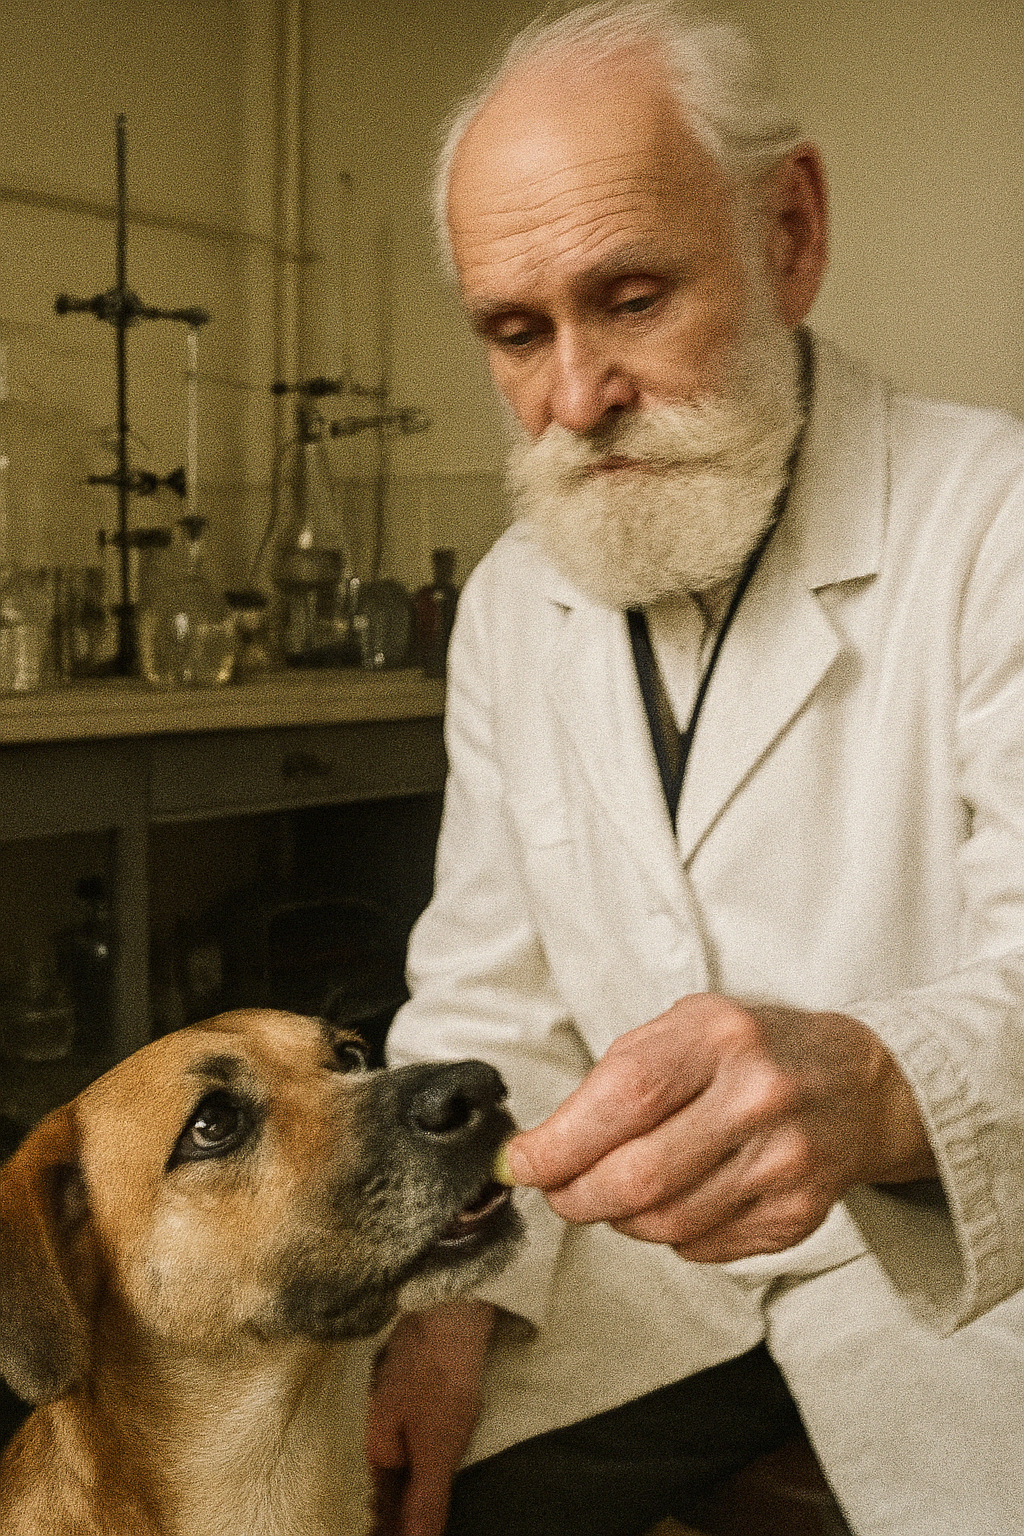
\includegraphics[width=0.8\textwidth]{figures/pawlows dog.png}}
\end{column}
\end{columns}

\end{frame}


\begin{frame}{What is Reinforcement Learning?}
\begin{itemize}
    \item  Reinforcement learning is also known as
\begin{itemize}
    \item  Optimal control
\item  Approximate dynamic programming
\item  Neuro-dynamic programming
 
\end{itemize} 
\end{itemize}
\begin{definition}
Reinforcement learning is an area of machine learning inspired by behavioral psychology, concerned with how software 
\textbf{\alt<2>{\textcolor{red1}{agents}}{\textcolor{black}{agents}}} ought to take 
\textbf{\alt<3-3>{\textcolor{red1}{actions}}{\textcolor{black}{actions}}} in an 
\textbf{\alt<4-4>{\textcolor{red1}{environment}}{\textcolor{black}{environment}}} so as to maximize some notion of cumulative 
\textbf{\alt<5-5>{\textcolor{red1}{reward}}{\textcolor{black}{reward}}}.
\end{definition}
\begin{itemize}
\item  \citet[][chapter 1]{sutton2018reinforcement}
\item  \citet[][chapter 1]{szepesvari2022algorithms}
\end{itemize}
    
\end{frame}



\begin{frame}{Reinforcement Learning Problem}

    \begin{center}

\begin{tikzpicture}[node distance=1cm]
\node[fill=lightgray!40!white,rectangle,draw,rounded corners=2pt,inner sep=1ex,line width=1.5pt,minimum height=0.8cm] (O) {\large Agent};
\node[draw,fill=lightgray!40!white,line width=1.5pt, rectangle,rounded corners=2pt,minimum height=1cm,below=of O] (A) {Environment};

%left Path connect
\draw[line width=1.2pt,latex-]  ([yshift=2mm]O.west) -- ++(-3,0) |- ([yshift=-2mm]A.west) node[pos=0.25,left,align=right,font=\scriptsize] { state\\ $S_t$};
\draw[line width=0.7pt,latex-]  ([yshift=-0.5mm]O.west) -- ++(-2.5,0) |- ([yshift=2.5mm]A.west) node[pos=0.25,right,align=left,font=\scriptsize] { reward\\ $R_t$};

%right Path connect
\draw[line width=1.2pt,-latex]  (O.east) -- ++(2.0,0) |- (A.east) node[pos=0.25,right,align=left,font=\scriptsize] {action\\ $A_t$};

\draw[-{Latex[scale=1.5]}] ([yshift=-2mm]A.west) -- ++(-1,0) node[pos=0.4,above=-1pt,font=\scriptsize] {$S_{t+1}$};
\draw[-{Latex[scale=1.2]}] ([yshift=2.5mm]A.west) -- ++(-1,0) node[pos=0.4,above=-1pt,font=\scriptsize] {$R_{t+1}$};


\draw[yshift=-1.9cm,xshift=-2.11cm,line width=1pt,densely dashed] (0,-0.5)--(0,0.5) node[below,pos=0,font=\scriptsize] {next step};
\end{tikzpicture}\\
\vspace{3mm}
  {Goal:} Learn to choose actions that maximize rewards

\end{center}
    
\end{frame}

\section{Applications and Examples}
{
\setbeamercolor{background canvas}{bg=BrewerBlue}
\begin{frame}
\centering
\Huge
\textcolor{white}{Applications and Examples}
\thispagestyle{empty}
\end{frame}
}

\begin{frame}{RL Examples}

\begin{itemize}
\item Game playing (go, atari, backgammon)
\item Elevator scheduling
\item Helicopter control
\item Spoken dialog systems
\item Data center energy optimization
\item Self-managing network systems
\item Autonomous vehicles
\end{itemize}
\end{frame}


\begin{frame}{RL Examples in the Social Sciences}

\begin{itemize}
\item Operations research\\ (pricing, vehicle routing)
\item Computational finance\\ (portfolio optimization, algorithmic trading)
\end{itemize}

\end{frame}


\begin{frame}{Operations Research}

\begin{columns}[T]
\begin{column}{0.55\textwidth}
\begin{itemize}
    \item  Example: vehicle routing

\item \textbf{Agent:} vehicle routing software
\item \textbf{Environment:} stochastic demand
\item \textbf{State:} vehicle location,  capacity and depot requests
\item \textbf{Action:} vehicle route
\item \textbf{Reward:} - travel costs 
\end{itemize}
\end{column}
\begin{column}{0.45\textwidth}
\centering
\includegraphics[width=0.9\textwidth]{figures/vehicle_routing.jpg}
\end{column}
\end{columns}
    
\end{frame}


\begin{frame}{Game Playing}
    \begin{columns}[T]
\begin{column}{0.5\textwidth}
\begin{itemize}
    \item  Example: Go (one of the oldest  and hardest board games)

\item \textbf{Agent:} player
\item \textbf{Environment:} opponent
\item \textbf{State:} board configuration
\item \textbf{Action:} next stone location
\item \textbf{Reward:} +1 win / -1 loose

 
\end{itemize}
\end{column}
\begin{column}{0.45\textwidth}
\centering
\includegraphics[width=0.7\textwidth]{figures/go_game2_move_37}
\end{column}
\end{columns}

\begin{itemize}
    \item  2016: AlphaGo defeats top player Lee Sedol (4-1)
\begin{itemize}
    \item 	Game 2 move 37: AlphaGo plays unexpected move (odds 1/10,000)\\
    \url{https://www.youtube.com/watch?v=WXuK6gekU1Y}
 
\end{itemize}
\end{itemize}
\end{frame}


\begin{frame}{Robotic Control}
    \begin{columns}[T]
\begin{column}{0.5\textwidth}
\begin{itemize}
    \item  Example: helicopter control

\item \textbf{Agent:} controller
\item \textbf{Environment:} helicopter
\item \textbf{State:} position, orientation,  velocity and angular velocity
\item \textbf{Action:} collective pitch, cyclic pitch, tail rotor control
\item \textbf{Reward:} - deviation from desired trajectory
 
\end{itemize}
\end{column}
\begin{column}{0.45\textwidth}
\centering
\includegraphics[width=0.9\textwidth]{figures/helicopter}
\end{column}
\end{columns}

\begin{itemize}
    \item  2008 (Andrew Ng): automated helicopter wins acrobatic  competition against humans\\
\url{https://www.youtube.com/watch?v=0JL04JJjocc}

\end{itemize}
\end{frame}

\begin{frame}{Conversational Agent}

    \begin{columns}[T]
\begin{column}{0.55\textwidth}
\begin{itemize}
\item  Example: Conversational Agent (ChatGPT)
\item  \textbf{Agent:} language model
\item \textbf{Environment:} user
\item \textbf{State:} conversation history
\item \textbf{Action:} next token 
\item \textbf{Reward:} ratings based on task completion, user satisfaction, etc.
\item \textbf{Today:} active area of research


\end{itemize}
\end{column}
\begin{column}{0.45\textwidth}
\centering
        \includegraphics[scale=0.30]{figures/conversational_agent.png}
\end{column}
\end{columns}
\end{frame}

\begin{frame}{Computational Finance}
\vspace{-11mm}
\begin{columns}[T]
\begin{column}{0.5\textwidth}
\begin{itemize}
    \item  Example: Automated trading

\item \textbf{Agent:} trading software
\item \textbf{Environment:} other traders
\item \textbf{State:} price history
\item \textbf{Action:} buy/sell/hold
\item \textbf{Reward:} amount of profit

\end{itemize}
\end{column}
\begin{column}{0.45\textwidth}
\centering
\includegraphics[width=1\textwidth]{figures/finance.png}
\end{column}
\end{columns}

\vspace{5mm}
    Example: trading strategies that adapt to real-time market signals

\end{frame}


\begin{frame}{RL Examples in the Social Sciences}
\textbf{Adaptive lab, field, or survey experiments}
\begin{itemize}
\item Advertising\pause
\item Educational learning\pause
\item Labor market platforms\pause
\item Public health interventions\pause
\item Social program targeting\pause
\item Crime prevention and policing\pause
\item Political campaign strategy\pause
\end{itemize}

\textbf{Explaining Behavior and Assisting Decision Making}
\begin{itemize}
\item Strategic decision making (game theory)\pause
\item Households choices (fertility, labor, education, consumption/saving)\pause
\item Firms choices (entry, exit, investments, hiring, pricing, output)
\end{itemize}
\end{frame}




\section{Course Overview}
{
\setbeamercolor{background canvas}{bg=BrewerBlue}
\begin{frame}
\centering
\Huge
\textcolor{white}{Course Overview}
\thispagestyle{empty}
\end{frame}
}

\begin{frame}{Course overview}
\begin{enumerate}
    \item Unit 1: Multi-Armed Bandits
    \item Unit 2: Markov Decision Processes\\
		\emph{Assignment 1}
		
    \item Unit 3: RL Algorithms\\
		\emph{Assignment 2}
		
    \item Unit 4: Deep RL
\end{enumerate}
\end{frame}

%% Unit 1
%\begin{frame}{Unit 1: Multi-Armed Bandits}
%\begin{itemize}
    %\item Multi-Armed Bandits
    %\item \(\varepsilon\)-greedy
    %\item Upper Confidence Bound
    %\item Thompson Sampling
    %\item Inference with Batched Bandits
    %\item Contextual Bandits
%\end{itemize}
%\end{frame}
%
%% Unit 2
%\begin{frame}{Unit 2: Markov Decision Processes}
%\begin{itemize}
    %\item Markov Processes
    %\item Markov Decision Processes
    %\item Bellman Equation
    %\item Value Iteration
    %\item Policy Iteration
%\end{itemize}\pause
%\vspace{0.5cm}
%\textbf{Assignment 1:}\\
%\small{Program a 40-Armed Bandit for the 40 DAX stocks that learns each day within the next two weeks the optimal share of investments in each stock.}
%\end{frame}
%
%% Break Slide
%\begin{frame}{Break}
%\vfill
%\centering
%\Large{\textit{Take a short break before we continue with Unit 3!}}
%\vfill
%\end{frame}
%
%% Unit 3
%\begin{frame}{Unit 3: Core RL Algorithms}
%\begin{itemize}
    %\item Overview of Reinforcement Learning
    %\item Monte Carlo Learning
    %\item Temporal Difference Learning
    %\item Q-Learning
    %\item On-policy vs. Off-policy Algorithms
%\end{itemize}\pause
%\vspace{0.5cm}
%\textbf{Assignment 2:}\\
%\small{Use 100 iterations to find the optimal policy for "The Cliff"—with achieving a target, a cost function, and the option of closing the business as an example.}
%\end{frame}
%
%% Unit 4
%\begin{frame}{Unit 4: Deep RL and Human Feedback}
%\begin{itemize}
    %\item Neural Networks
    %\item Deep Neural Networks
    %\item Deep Q-Learning
    %\item Proximal Policy Optimization
    %\item Reinforcement Learning through Human Feedback
%\end{itemize}
%\end{frame}
%
%
%\section{Prerequisites}
%
%\begin{frame}{Prerequisites}
%\renewcommand{\baselinestretch}{1}
%
%A curious mind.
%
%\end{frame}
%

\begin{frame}[t,allowframebreaks
]\nocite{*}
\frametitle{References}
\small
\bibliography{bib}
\end{frame}


\section{Takeaways}
{
\setbeamercolor{background canvas}{bg=BrewerBlue}
\begin{frame}
\centering
\Huge
\textcolor{white}{Takeaways}
\thispagestyle{empty}
\end{frame}
}

\begin{frame}{What is Reinforcement Learning?}

\begin{itemize}
\item  Comprehensive, but challenging form of machine learning
\begin{itemize}
\item Interdependent sequence of decisions
\item Incomplete model
\item Stochastic environment
\item No supervision
\item Partial and delayed feedback 
 
\end{itemize}
\item  \textbf{Long term goal:} autonomous agents---without needing explicit supervision (according to ChatGPT)

    \end{itemize}
\end{frame}

\end{document}
